\noindent To determine whether the child branches across the network are either "RBC-enriched" or "RBC- depleted", Q$^{*}_{blood}$ and Q$^{*}_{rbc}$ were evaluated first before considering the sign and magnitude of $\Delta$Q$^{*}$ $=$ Q$^{*}_{rbc}$ $-$ Q$^{*}_{blood}$. (Refer back to Section \ref{Post_Processing} for definitions and equations of variables here. E.g. Q$^{*}_{blood}$) If the RBCs were distributed in proportional to the blood flow, it implies that $\Delta$Q$^{*}$ $=$ 0 which shows a linear relationship between Q$^{*}_{blood}$ and Q$^{*}_{rbc}$. For "RBC-enriched" branches, Q$^{*}_{rbc}$ > Q$^{*}_{blood}$ as this indicates that the child branch has more RBCs than linear allocation. Whereas when Q$^{*}_{rbc}$ < Q$^{*}_{blood}$, the child branch is referred to as an "RBC-depleted" branch given that the child branch has fewer RBCs than the linear hypothesis. \\


\noindent Based on the given simulation data, several branches were found without any presence of RBCs. This raises a critical question on what are the governing factors that could influence the blood flow in microvascular networks. Although it is natural to think that very narrow branches (smaller than the diameter of a human RBC) should restrict RBCs from passing through, several studies\cite{FreundJonathanB2013Tfor, Salehyar2017EffectsOS, LuHuijie2019Biso} have shown that highly deformable RBCs under physiological conditions allows them to pass through extremely confined branches with diameters even as small as 1$-$2 $\mu$m.


\subsubsection{Geometric \& Hydrodynamic Diameters}
\noindent For all of the child branches examined in this data analysis (46 in total, Figure \ref{DisproportionalityIndexDs}), it was observed that RBC depletion occurs throughout the entire range of both geometric and hydrodynamic branch diameters, whereas RBC enrichment occurs only when D$_{G}$ and D$_{H}$ are greater than 6.7 $\mu$m. In addition to this, one specific child branch with D$_{G}$ $\approx$ 10.5 $\mu$m (larger than the diameter of an RBC) had a disproportionality index of $-$0.21 which indicates a 21$\%$ reduction in RBC transit in that child branch. This shows that RBC depletion in the micro-vascular network cannot be purely based on geometric measurements of the network and hence, it is not a size-exclusion effect. Last but not least, for branch diameters between 6.7 $\mu$m and 14 $\mu$m, the branches have almost equivalent probabilities of being either enriched or depleted. Therefore, the branch diameters (D$_{G}$ and D$_{H}$) obtained from the given simulation data indicate that branch diameters alone do not differentiate the RBC enrichment or depletion apart as shown in Figure \ref{DisproportionalityIndexDs}. This also demonstrates that branch diameter is not the primary factor affecting RBC transits in microvascular networks. (Refer back to Section \ref{Post_Processing} for the methods of calculating D$_{G}$ and D$_{H}$)

\begin{figure}[H]
\centering
\begin{subfigure}{0.48 \textwidth}
    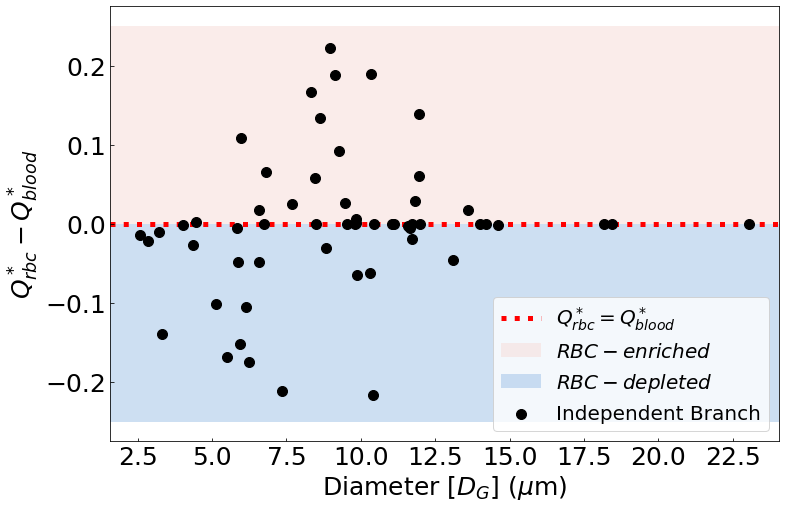
\includegraphics[width=1\textwidth]{images/DisproportionalityIndexDG.png}
    \caption{\textit{Average Geometric Diameters} \label{DisproportionalityIndexDG}}
\end{subfigure}
\hfill
\begin{subfigure}{0.48 \textwidth}
    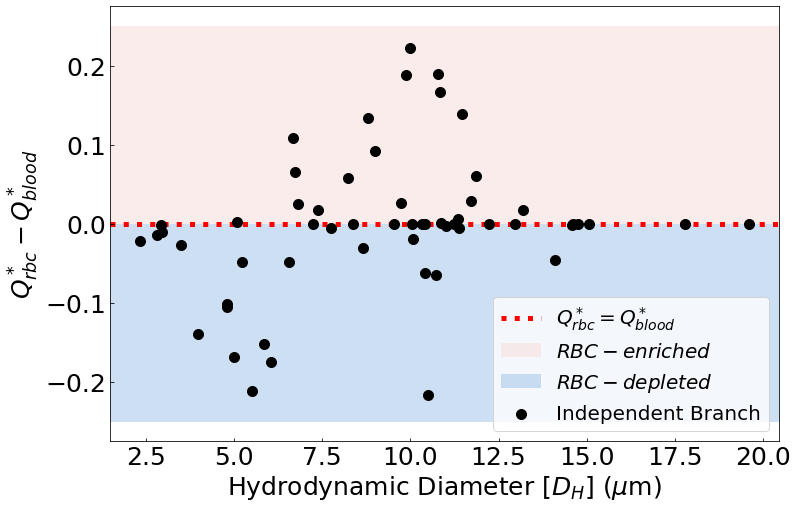
\includegraphics[width=1\textwidth]{images/DisproportionalityIndexDH.png}
    \caption{\textit{Evaluated Hydrodynamic Diameters} \label{DisproportionalityIndexDH}}
\end{subfigure}
\caption{\textit{Quantification of RBC enrichment and depletion in micro-vascular networks based on branch diameters. Q$^{*}_{blood}$ and Q$^{*}_{rbc}$ represent the normalised blood flow and RBC flux in a child branch relative to its parent branch in each bifurcation respectively. $\Delta$Q$^{*}$ $=$ Q$^{*}_{rbc}$ $-$ Q$^{*}_{blood}$ represents an index that describes the disproportionality of RBC partitioning where the sign of $\Delta$Q$^{*}$ indicates which branches are classified as "RBC-depleted" (negative $\Delta$Q$^{*}$, blue region) and "RBC-enriched" (positive $\Delta$Q$^{*}$, red region).} \label{DisproportionalityIndexDs}}
\end{figure}

\subsubsection{Discharge Haematocrit}
\begin{figure}[H]
\centering
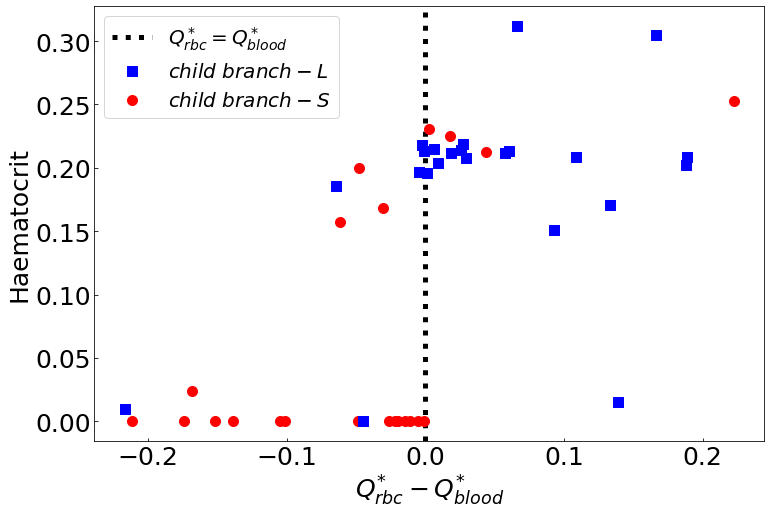
\includegraphics[width=0.65\textwidth]{images/DisproportionalityIndexHD.png}
\caption{\textit{Network level inspection of RBC enrichment (right-hand region) / RBC depletion (left-hand region) based on haematocrit. The "L"/"S" indicate the relatively larger (blue squares) / smaller (red circles) child branches in each of the investigated bifurcations across the networks respectively. The black dotted line represents Q$^{*}_{blood}$ $=$ Q$^{*}_{rbc}$.} \label{DisproportionalityIndexHD}}
\end{figure}

\noindent Meanwhile, discharge haematocrit (H$_{D}$) is another important factor for consideration to determine the effects of RBC transits across the microvascular networks. Based on Figure \ref{DisproportionalityIndexHD} above, it was observed that the majority of the close-to-zero haematocrit child branches are "RBC-depleted" although there are a few child branches spotted experiencing RBC depletion even with an average haematocrit of around 18\%. The range of H$_{D}$ in the RBC enrichment region except for one single outlier was found between 0.15 and 0.31. Last but not least, it is evident that the majority of the larger and smaller child branches are within the RBC enrichment and RBC depletion regions respectively. Therefore, in accordance with these findings, we can conclude that neither discharge haematocrit nor branch diameter alone is able to distinctively predict which branches are categorised as either "RBC-depleted" or "RBC-enriched". Furthermore, although the majority of the larger and smaller child branches lie within the RBC-enrichment and RBC-depletion regions respectively, there are still several anomalies that suggest that both the discharge haematocrit and branch diameter should be simultaneously considered instead. Kindly note that the context of "larger" and "smaller" (CB-L and CB-S) in the entire dissertation is a comparative notion between the two child branches in each bifurcation and not a measure of the absolute branch diameter. 

